\section{Results}
\label{sec:results}

All numbers come from the full-study run records, scored by the frozen parser and placeholder rules except where marked post hoc.
Unless stated, they are on documents with $n < k$ at $k = 3$ and 5; 95\% group-bootstrap intervals are in the tables of contrasts.

\subsection{A shown minimum, per model}
\label{sec:main}

\begin{table*}[t]
  \centering
  \small
  \begin{adjustbox}{max width=\linewidth}\begin{tabular}{lrrrrr}
  \toprule
  Model & C1 & C2 & C3 & C4 & C5 \\
  \midrule
  Qwen3.5-0.8B & $-0.38$ [$-0.84$, $+0.07$] & $-0.59$ [$-1.06$, $-0.13$] & $-0.32$ [$-0.73$, $+0.08$] & $-0.63$ [$-0.77$, $-0.49$] & $-0.31$ [$-0.47$, $-0.16$] \\
  Qwen3.5-2B & $+0.12$ [$-1.39$, $+1.56$] & $+0.60$ [$-0.51$, $+1.72$] & $+2.13$ [$+1.22$, $+3.07$] & $-0.44$ [$-0.74$, $-0.13$] & $-0.22$ [$-0.32$, $-0.11$] \\
  Qwen3.5-9B & $+0.51$ [$+0.39$, $+0.65$] & $+0.62$ [$+0.50$, $+0.74$] & $+0.80$ [$+0.69$, $+0.92$] & $+0.11$ [$+0.06$, $+0.15$] & $-0.64$ [$-0.81$, $-0.53$] \\
  Qwen3.5-27B & $+1.20$ [$+1.07$, $+1.33$] & $+1.24$ [$+1.11$, $+1.37$] & $+1.29$ [$+1.18$, $+1.41$] & $+0.37$ [$+0.32$, $+0.41$] & $-0.57$ [$-0.61$, $-0.53$] \\
  Gemma 4 31B & $+1.13$ [$+0.99$, $+1.27$] & $+1.68$ [$+1.55$, $+1.81$] & $+1.70$ [$+1.57$, $+1.83$] & $+0.93$ [$+0.87$, $+0.99$] & $-0.66$ [$-0.70$, $-0.62$] \\
  Olmo 3.1 32B & $+0.47$ [$+0.29$, $+0.64$] & $+0.26$ [$+0.10$, $+0.42$] & $+1.20$ [$+1.00$, $+1.42$] & $+0.02$ [$-0.05$, $+0.08$] & $-0.64$ [$-0.73$, $-0.56$] \\
  Ministral 3 14B & $+1.03$ [$+0.87$, $+1.19$] & $+0.30$ [$+0.12$, $+0.45$] & $+1.13$ [$+0.99$, $+1.27$] & $+0.19$ [$+0.14$, $+0.24$] & $-0.94$ [$-1.00$, $-0.88$] \\
  gpt-oss-20b & $+0.83$ [$+0.65$, $+1.01$] & $+0.87$ [$+0.72$, $+1.01$] & $+0.98$ [$+0.86$, $+1.10$] & $+0.28$ [$+0.23$, $+0.33$] & $-0.32$ [$-0.38$, $-0.27$] \\
  \midrule
  Pooled & $+0.61$ [$+0.42$, $+0.80$] & $+0.62$ [$+0.46$, $+0.78$] & $+1.11$ [$+0.97$, $+1.25$] & $+0.10$ [$+0.06$, $+0.15$] & $-0.54$ [$-0.58$, $-0.50$] \\
  \bottomrule
\end{tabular}
\end{adjustbox}
  \caption{Confirmatory contrasts per GPU model and pooled (8 models, Holm $p < 0.0001$ for each pooled contrast). C1: \cnd{min\_k\_shown} at $k = 5$ minus $k = 3$ ($n \leq 2$). C2: \cnd{min\_k\_shown} minus \cnd{none}, the main measure. C3: \cnd{min\_k\_shown} minus \cnd{max\_k\_shown}. C4: \cnd{prose\_exactly\_k} minus \cnd{prose\_up\_to\_k}, five wordings averaged. C1 to C4 in substantive entries per output; C5: \cnd{min\_k\_escape} minus \cnd{min\_k\_enforced}, excess entries per forced slot. 95\% intervals from 10,000 bootstrap draws over document groups.}
  \label{tab:permodel}
\end{table*}

A minimum shown in the schema lengthens lists for six of the eight GPU models, by 0.26 (Olmo 3.1 32B) to 1.68 entries (Gemma 4 31B), each with an interval above 0 (Table~\ref{tab:permodel}, column C2).
Pooled over the eight, it adds 0.62 entries [0.46, 0.78] and raises over-count by 20.9 points [19.5, 22.3]: on the same documents, about one more list in five runs past the true count.
The estimate holds without the pilot documents, under the mixed model, with the five families weighted equally and with any one family left out (0.47 to 0.78; Appendices~\ref{app:generality} and~\ref{app:perset}).

The two smallest models are the exceptions.
Qwen3.5-2B lengthens its lists ($+0.60$), but its interval spans 0.
Qwen3.5-0.8B often writes no readable list: 36.6\% of its outputs are unreadable, mostly an answer written inside a copy of the schema, which the frozen rules count as 0 entries, so its estimate turns negative ($-0.59$; Appendix~\ref{app:outcomes}).
Read with a lenient parser, it over-counts on about half its outputs both with no count and under a shown minimum (post hoc; Appendix~\ref{app:posthoc}).
Because unreadable outputs count as empty lists, this model pulls the pooled numbers down: without it, the main contrast is $+0.80$ entries [0.63, 0.96] and over-count rises from 35.0\% to 59.8\% (post hoc).
The registered pooled estimate is therefore the conservative one.

The added entries are not true items that the no-count list missed: the share of true items left out (documents with $n \geq 1$) is 18.2\%\pre{} under a shown minimum and 17.0\%\pre{} with no count (Table~\ref{tab:outcomes}).
Over all documents, an enforced minimum misses the fewest true items (recall 0.91\pre{}, against 0.83\pre{} with no count) because it adds the most entries, and prose ``up to $k$'' has the best entry F1 (0.60\pre{}, against 0.53\pre{}; post hoc, Table~\ref{tab:prf}).

The other confirmatory contrasts agree (Table~\ref{tab:permodel}).
Raising the shown minimum from 3 to 5 on the same document adds 0.61 entries (C1), about 0.3 per added slot; over-count barely moves, since a list already above $n$ at $k = 3$ cannot over-count twice, which is why the registered outcome is length.
A shown minimum gives 1.11 entries more than a shown maximum (C3), though this sums two opposite effects ($+0.62$ and $-0.49$ against no count).
In prose, ``exactly $k$'' gives 0.10 entries and 8.2 over-count points more than ``up to $k$'' (C4).

A count in prose pulls lists toward $k$ from both sides.
In every wording, both prose conditions shorten lists against no count ($-0.43$ to $-1.02$ entries; Table~\ref{tab:wordings}), mostly by cutting long lists, yet the share that over-counts rises from 34.5\% to 42.7\% for ``up to $k$'' and 50.9\% for ``exactly $k$'' (Table~\ref{tab:outcomes}).
A mean length change can therefore hide padding, which is why over-count is reported beside it.
The prose conditions also replace the ``List all'' instruction, so part of their difference from no count may come from the wording rather than the count.

The effect holds with the annotators' original counts, on documents whose list the cleanup kept or changed, and on $n = 0$ as on $n \geq 1$ documents (Appendix~\ref{app:key}).
By set, contrast 2 runs from $+0.07$ (Wikipedia people) to $+1.54$ entries (job-ad skills), and over-count rises in all nine sets, by 6.5 to 31.2 points (Appendix~\ref{app:perset}).

\subsection{Registered controls and the empty-document test}
\label{sec:named}

\begin{table}[t]
  \centering
  \small
  \setlength{\tabcolsep}{3pt}
  \begin{adjustbox}{max width=\linewidth}
  \begin{tabular}{@{}llr@{}}
    \toprule
    Test & Unit & Estimate [95\% CI] \\
    \midrule
    \rows{generated/tab_named_rows.tex}
    \bottomrule
  \end{tabular}
  \end{adjustbox}

  \vspace{6pt}
  \begin{adjustbox}{max width=\linewidth}
  \begin{tabular}{@{}lrr@{}}
    \toprule
    Empty documents, $k = 1$ & $\geq 1$ entry \% & vs \cnd{none} (pts) \\
    \midrule
    \rows{generated/tab_empty_rows.tex}
    \bottomrule
  \end{tabular}
  \end{adjustbox}
  \caption{Registered controls and the empty-document test, eight GPU models pooled. Top: documents with $n < k$, $k = 3$ and 5, except the two $n \geq k$ rows ($k = 1$, 3 and 5); $n < k$ minus $n \geq k$ is the change on $n < k$ documents minus the change on $n \geq k$ documents. Bottom: the 105 documents with no true item at $k = 1$, share of outputs with at least one substantive entry. \pre{} rests on the matcher. Per model: Appendix~\ref{app:named}.}
  \label{tab:named}
\end{table}

\paragraph{Fewer is fine.}
Adding ``If the document contains fewer than $k$, list all available ones.'' reverses the effect: lists end 0.77 entries shorter than with no count, and over-count falls 3.5 points below the no-count level (Table~\ref{tab:named}).
Seven of the eight models shorten their lists against the plain shown minimum, though Qwen3.5-27B still lists 0.46 entries more than with no count (Appendix~\ref{app:named}).
The line has a cost: the share of true items left out rises from 17.0\%\pre{} to 24.3\%\pre{} (Table~\ref{tab:outcomes}).

\paragraph{Enough items.}
On documents that already hold at least $k$ true items, a shown minimum does not lengthen lists ($-0.15$ entries [$-0.30$, $-0.02$]) and leaves true items left out unchanged.
On $n < k$ documents its effect exceeds this by 0.93 entries: the effect comes from filling the forced slots.

\paragraph{Empty documents at $k = 1$.}
On the 105 documents with no true item, even \texttt{minItems: 1}, which asks only for a non-empty list, raises the share of outputs with at least one substantive entry from 34.9\% with no count by 7.4 points when shown, and by 47.5 points, to 82.4\%, when enforced.
The ``fewer is fine'' line and the N/A escape both bring it below the no-count level.

\paragraph{maxItems.}
A shown maximum is not neutral: it shortens lists against no count ($-0.49$ entries [$-0.61$, $-0.37$]), so it fails the protocol's test for a harmless maximum.
It barely changes over-count (35.7\% against 34.5\%) but leaves out more true items (20.9\%\pre{} against 17.0\%\pre{}).

\subsection{What the lists hold}
\label{sec:what}

\begin{figure}[t]
  \centering
  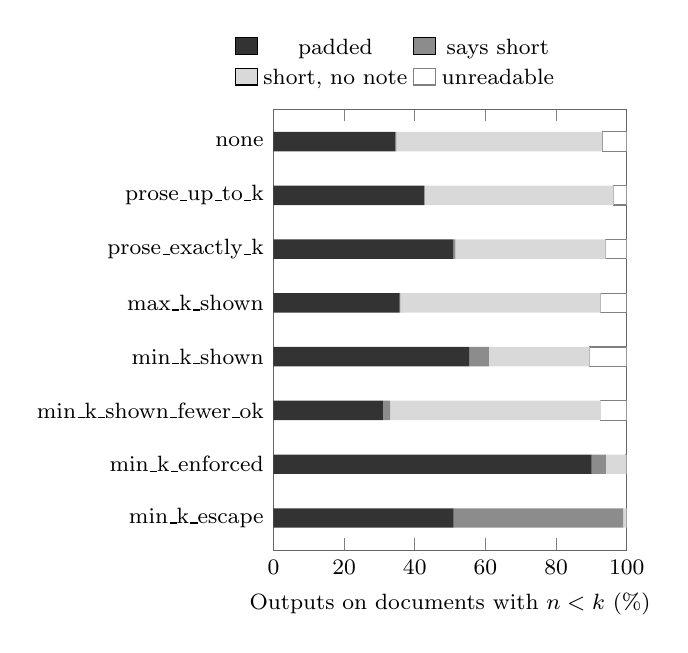
\begin{tikzpicture}
    \begin{axis}[xbar stacked, scale only axis, width=0.37\columnwidth, height=5.6cm, bar width=7pt,
                 xmin=0, xmax=100, xlabel={Outputs on documents with $n < k$ (\%)},
                 ytick={1,...,8}, ymin=0.4, ymax=8.6,
                 yticklabels={\cnd{min\_k\_escape}, \cnd{min\_k\_enforced}, \cnd{min\_k\_shown\_fewer\_ok}, \cnd{min\_k\_shown}, \cnd{max\_k\_shown}, \cnd{prose\_exactly\_k}, \cnd{prose\_up\_to\_k}, \cnd{none}},
                 y tick label style={font=\footnotesize}, x tick label style={font=\footnotesize},
                 label style={font=\footnotesize}, axis line style={black!60},
                 legend style={font=\footnotesize, draw=none, at={(0.35,1.02)}, anchor=south, legend columns=2}]
      \addplot[fill=black!80, draw=none] coordinates {(51.0,1) (90.1,2) (31.0,3) (55.4,4) (35.7,5) (50.9,6) (42.7,7) (34.5,8)};
      \addplot[fill=black!45, draw=none] coordinates {(48.0,1) (4.0,2) (2.0,3) (5.6,4) (0.2,5) (0.6,6) (0.1,7) (0.3,8)};
      \addplot[fill=black!15, draw=none] coordinates {(0.9,1) (5.7,2) (59.7,3) (28.5,4) (56.7,5) (42.5,6) (53.5,7) (58.3,8)};
      \addplot[fill=white, draw=black!50] coordinates {(0.1,1) (0.2,2) (7.3,3) (10.5,4) (7.3,5) (6.0,6) (3.7,7) (6.9,8)};
      \legend{padded, says short, {short, no note}, unreadable}
    \end{axis}
  \end{tikzpicture}
  \caption{How outputs on documents with $n < k$ end, by condition, eight GPU models pooled, $k = 3$ and 5. Padded: more substantive entries than $n$, even with a note. All columns: Table~\ref{tab:outcomes}.}
  \label{fig:sorting}
\end{figure}



Over-count is not zero without a count: 34.5\% of no-count outputs on $n < k$ documents already list more than $n$ substantive entries, mostly grounded padding (64.6\%\pre{}; Table~\ref{tab:fillfull}).
This is ordinary extraction error, and each paired contrast measures what a condition adds to it on the same document and model.
On the documents a model gets exactly right with no count, a shown minimum makes 35.2\% [33.0, 37.5] of its lists pad, against 5.0\% under a shown maximum (post hoc; Table~\ref{tab:cleanbase}).
A shown minimum moves lists toward $k$: the share with exactly $k$ entries rises from 5.6\% to 35.5\%, and 55.4\% of outputs pad (Figure~\ref{fig:sorting}).
Enforced, the minimum leaves 0.6\% of lists short of $k$ and 90.1\% padded.
That much follows from the decoder, which all but rules out a shorter list; what the enforced condition shows is what fills the slots.

Most extra entries are grounded padding: 62.9\%\pre{} under a shown minimum and 79.6\%\pre{} under an enforced one, as in Figure~\ref{fig:example}.
Most of the rest are invented: 29.5\%\pre{} under a shown minimum, about the share with no count (29.8\%\pre{}), so the minimum adds both kinds in the proportions they already have; corrected with the authors' labels, the invented share is 23.4\% (post hoc; Appendix~\ref{app:posthoc}).
That makes the padding hard to catch: a source check removes invented entries, but 46.6\%\pre{} of all extra entries under a shown minimum pass it (post hoc).

\paragraph{The N/A escape (C5).}
Offering ``N/A'' under an enforced minimum cuts the excess entries per forced slot by 0.54 (rate ratio 0.57 in the Poisson mixed model), and every GPU model's own estimate is below 0 (Table~\ref{tab:permodel}).
It is not a full fix: 51.0\% of outputs still pad, and the two smallest models barely use it (Qwen3.5-0.8B still pads 89.6\% of its outputs and Qwen3.5-2B 83.0\%; Appendix~\ref{app:outcomes}).

\subsection{Hosted models and serving stack}
\label{sec:hosted}

All nine hosted runs lengthen their lists under a shown minimum, by 0.28 (Ministral 3 14B on Bedrock) to 2.39 entries (DeepSeek V3.2; Figure~\ref{fig:headline}), and give more entries under a minimum than under a maximum (Table~\ref{tab:hosted}).
For four of them (both DeepSeek models, Kimi K3 and Qwen3-235B), the ``fewer is fine'' line does not undo the effect: they still list 0.30 to 0.53 entries more than with no count.
The serving stack does not drive the result: for the three models run both on the GPU and hosted, the main contrast differs by at most 0.04 entries and 1.1 over-count points, within the registered limit of 10 points.

\subsection{Exploratory: re-asking and thinking}
\label{sec:exploratory}

\paragraph{Re-asking.}
Libraries that validate a schema send a failing reply back with the validation error.
We did this once for every shown-minimum reply shorter than $k$, in five runs (four models, with Ministral 3 14B both on the GPU and on Bedrock).
Over-count among the re-asked outputs rose in every run: from 10.0\% to 69.0\% for Qwen3.5-9B and from 14.0\% to 78.3\% for Kimi K3 (Appendix~\ref{app:reask}).
The error restates the minimum, so complying with it is expected.
The point is practical: after the default retry, 44.0 to 81.6\% of these short lists, truthful ones included, are padded.
A re-ask that adds ``fewer is fine'' was not tested.

\paragraph{Thinking.}
Thinking does not help (Appendix~\ref{app:thinking}, Table~\ref{tab:thinking}).
For Qwen3.5-9B it makes padding worse: in each of three request seeds, contrast 2 is 1.1 to 1.2 entries larger with thinking on, and over-count under a shown minimum rises from 43--47\% to 81--83\%.
Kimi K3 moves the same way, less ($+0.58$ entries on the pilot documents; its pair also differs in temperature).
Gemma 4 31B shows no length effect ($-0.11$ [$-0.23$, 0.01]), though its over-count under a shown minimum rises from 61.8\% to 66.1\%.
The thinking often names the shortfall, in 88--89\% of Qwen3.5-9B's padded outputs by a phrase search, and the model pads anyway.
